\begin{refsection} % refsection environment
\chapter[Short title]{Long title}

\section{Introduction}
Lorem ipsum dolor sit amet, consectetur adipiscing ...
We used the \acrfull{mwm} to test for spatial learning. However, with the \acrshort{mwm}, we... and \acrshort{mmmmmm} and \acrshort{rm}
\section{Methods}
Lorem ipsum dolor sit amet, consectetur adipiscing ... And \acrfull{rm} for... \acrfull{mmmmmm} and with \acrshort{mwm}
and \acrlong{mmmmmm} and \acrshort{rm2} and \acrshort{rm3} and \acrshort{orm}
\section{Results} 
And here we cite \cite{Famoye2015}. And also \citeauthor{Famoye2015}. 

The table \ref{table:1} is an example of referenced \LaTeX elements.

\begin{table}[h!]
	\centering
	\begin{tabular}{||c c c c||} 
		\hline
		Col1 & Col2 & Col2 & Col3 \\ [0.5ex] 
		\hline\hline
		1 & 6 & 87837 & 787 \\ 
		2 & 7 & 78 & 5415 \\
		3 & 545 & 778 & 7507 \\
		4 & 545 & 18744 & 7560 \\
		5 & 88 & 788 & 6344 \\ [1ex] 
		\hline
	\end{tabular}
	\caption{Table to test captions and labels}
	\label{table:1}
\end{table}

\begin{figure}[ht]
	\centering
	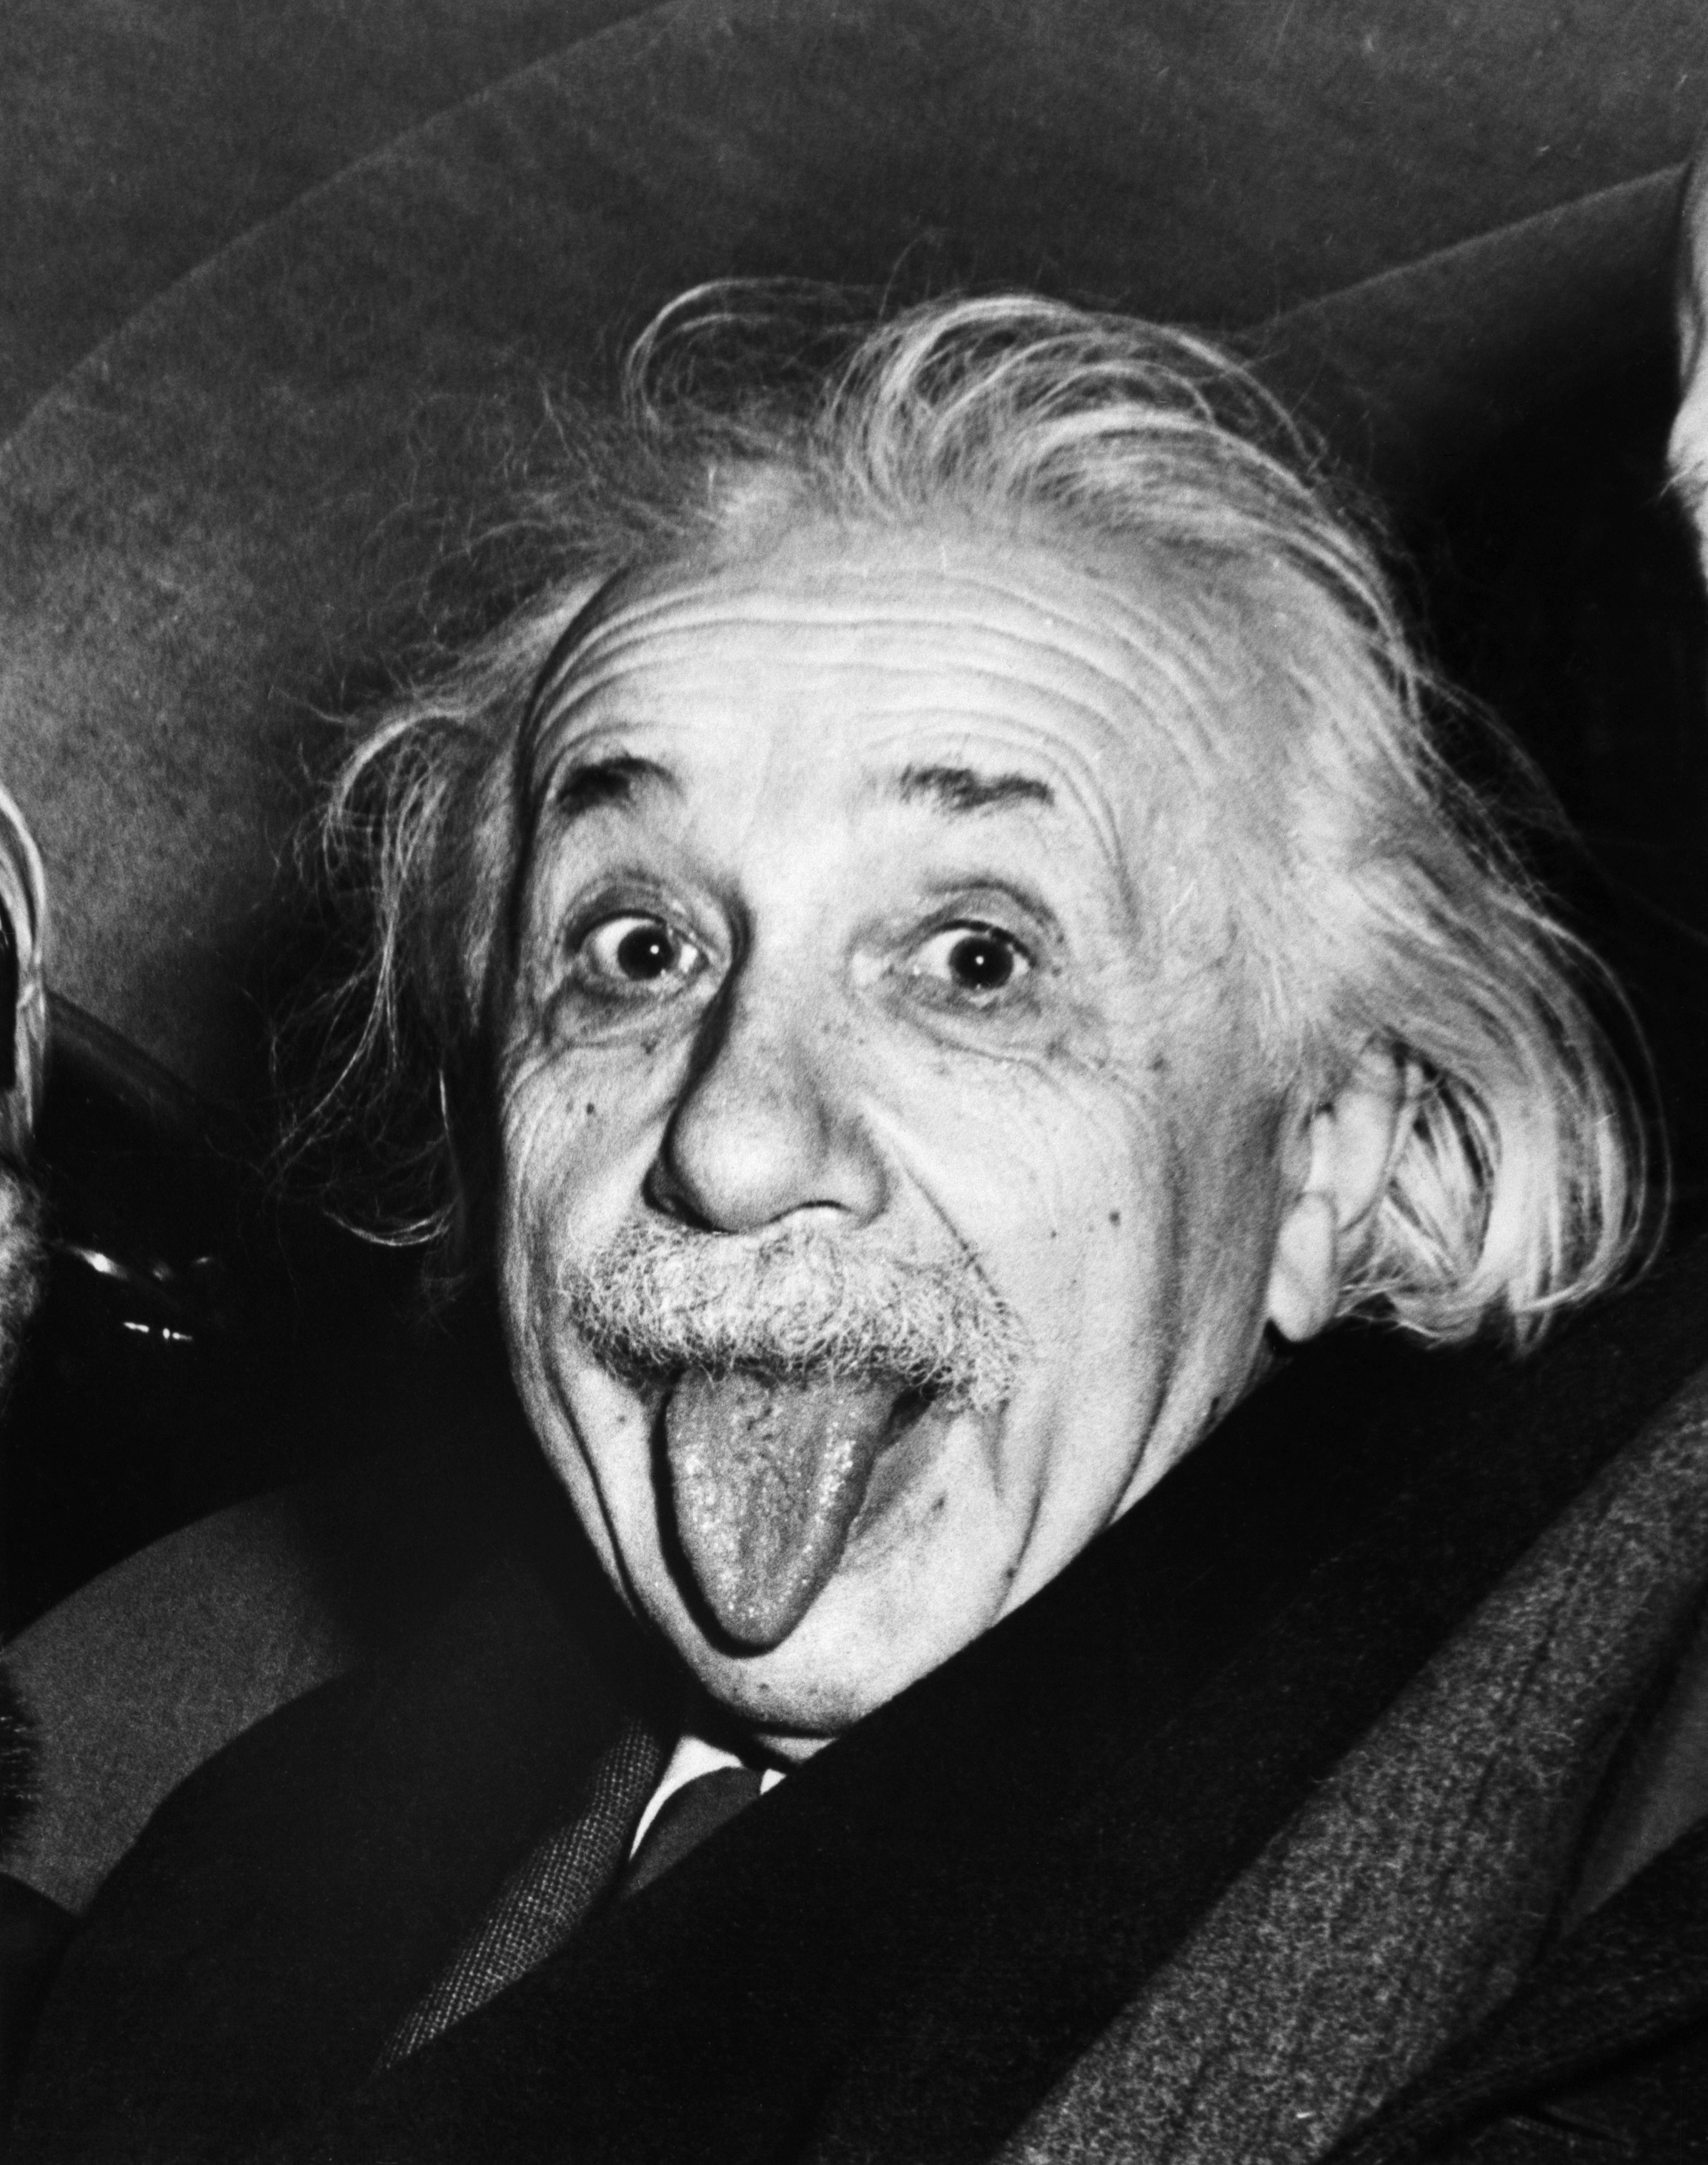
\includegraphics[width=\textwidth]{einstein.jpg}
	\caption[Einstein]{Einstein, a German-born theoretical physicist.}
	\centering
	\label{fig:1}
\end{figure}

As you can see in the photo \ref{fig:1}, ... Also, in page \pageref{fig:1}  we can see...

"But I must explain to you how all this mistaken idea of denouncing pleasure and praising pain was born and I will give you a complete account of the system, and expound the actual teachings of the great explorer of the truth, the master-builder of human happiness. No one rejects, dislikes, or avoids pleasure itself, because it is pleasure, but because those who do not know how to pursue pleasure rationally encounter consequences that are extremely painful. Nor again is there anyone who loves or pursues or desires to obtain pain of itself, because it is pain, but because occasionally circumstances occur in which toil and pain can procure him some great pleasure. To take a trivial example, which of us ever undertakes laborious physical exercise, except to obtain some advantage from it? But who has any right to find fault with a man who chooses to enjoy a pleasure that has no annoying consequences, or one who avoids a pain that produces no resultant pleasure?"

\subsection[SubShort]{Long title subsection}
This is a subsection
\subsubsection[SubSubShort]{Long title subsubsection}
This is a subsubsection
\paragraph{Paragraph title}
This is a paragraph
\subparagraph{Subparagraph title}
This is a subparagrah. "But I must explain to you how all this mistaken idea of denouncing pleasure and praising pain was born and I will give you a complete account of the system, and expound the actual teachings of the great explorer of the truth, the master-builder of human happiness. No one rejects, dislikes, or avoids pleasure itself, because it is pleasure, but because those who do not know how to pursue pleasure rationally encounter consequences that are extremely painful. Nor again is there anyone who loves or pursues or desires to obtain pain of itself, because it is pain, but because occasionally circumstances occur in which toil and pain can procure him some great pleasure. To take a trivial example, which of us ever undertakes laborious physical exercise, except to obtain some advantage from it? But who has any right to find fault with a man who chooses to enjoy a pleasure that has no annoying consequences, or one who avoids a pain that produces no resultant pleasure?"

"But I must explain to you how all this mistaken idea of denouncing pleasure and praising pain was born and I will give you a complete account of the system, and expound the actual teachings of the great explorer of the truth, the master-builder of human happiness. No one rejects, dislikes, or avoids pleasure itself, because it is pleasure, but because those who do not know how to pursue pleasure rationally encounter consequences that are extremely painful. Nor again is there anyone who loves or pursues or desires to obtain pain of itself, because it is pain, but because occasionally circumstances occur in which toil and pain can procure him some great pleasure. To take a trivial example, which of us ever undertakes laborious physical exercise, except to obtain some advantage from it? But who has any right to find fault with a man who chooses to enjoy a pleasure that has no annoying consequences, or one who avoids a pain that produces no resultant pleasure?"

"But I must explain to you how all this mistaken idea of denouncing pleasure and praising pain was born and I will give you a complete account of the system, and expound the actual teachings of the great explorer of the truth, the master-builder of human happiness. No one rejects, dislikes, or avoids pleasure itself, because it is pleasure, but because those who do not know how to pursue pleasure rationally encounter consequences that are extremely painful. Nor again is there anyone who loves or pursues or desires to obtain pain of itself, because it is pain, but because occasionally circumstances occur in which toil and pain can procure him some great pleasure. To take a trivial example, which of us ever undertakes laborious physical exercise, except to obtain some advantage from it? But who has any right to find fault with a man who chooses to enjoy a pleasure that has no annoying consequences, or one who avoids a pain that produces no resultant pleasure?"


\section{Discussion}

\addcontentsline{toc}{section}{References}
\printbibliography[heading=subbibliography, title={References}] % print section bibliography
\end{refsection}
